% Author :  Lionel du Peloux
% Contact : lionel.dupeloux@gmail
% Year : 2017

% ===========================
% COMPILER DIRECTIVES
% ===========================
% !TEX encoding = UTF-8 Unicode
% !TEX TS-program = XeLaTeX-shellescape
% !BIB TS-program = biber
% !BIB program = biber


\PassOptionsToPackage{showrules}{blurb}
% \PassOptionsToPackage{showframe}{blurb}
\PassOptionsToPackage{showbleed}{blurb}
% \PassOptionsToPackage{showcanon}{blurb}
% \PassOptionsToPackage{nobleed}{blurb}
\PassOptionsToPackage{cover}{blurb}

\documentclass[12pt,fleqn]{thesis}
	\graphicspath{{./ch7_numeric/img/}{./ch6_kirchhoff/img/}{./ch5_energy/img/}{./ch4_geometry/img/}{./ch3_creteil/img/}{./ch2_gridshell/img/}{./cover/}}
	\addbibresource{library.bib}

\usepackage{multicol}

\newlength\MainBarYOffset
\newlength\MainBarHeight
\newlength\MainBarStepWidth
\newlength\MainTextXMargin
\newlength\AuthorYMargin
\newlength\AuthorWidth
\newlength\AuthorRuleWidth
%
\setlength{\MainBarYOffset}{\PageHeight/2}
\setlength{\MainBarHeight}{2.5cm}
\setlength{\MainBarStepWidth}{2cm}
\setlength{\MainTextXMargin}{2cm}
%
\setlength{\AuthorYMargin}{1.5cm}
\setlength{\AuthorRuleWidth}{4mm}

% FONT FAMILY
\newfontfamily\FTRegular{FuturaLT}[Scale = MatchUppercase]
\newfontfamily\FTLight{FuturaLT-Light}[Scale = MatchUppercase]
\newfontfamily\FTBold{FuturaLT-Bold}[Scale = MatchUppercase]
\newfontfamily\FTHeavy{FuturaLT-Heavy}[Scale = MatchUppercase]
\newfontfamily\GSLight{GillSans-Light}[Scale = MatchUppercase]

% TYPE FACE
\DeclareRobustCommand{\tfgridshell}{\FTBold\fontsize{70pt}{0pt}\selectfont}
\DeclareRobustCommand{\tfelastica}{\FTLight\fontsize{60pt}{0pt}\selectfont}
\DeclareRobustCommand{\tfauthor}{\FTRegular\fontsize{16pt}{0pt}\selectfont}
\DeclareRobustCommand{\tfyear}{\FTHeavy\fontsize{25pt}{0pt}\selectfont}
\DeclareRobustCommand{\tfphd}{\FTHeavy\fontsize{30pt}{0pt}\selectfont}
\DeclareRobustCommand{\tftxt}{\GSLight\small}

\usepackage{adjustbox}

\begin{document}
\thispagestyle{empty}
\AddToShipoutPictureBG*{%
	\begin{tikzpicture}[remember picture, overlay, inner sep=0pt]
		% main bar nodes
		\path (PGtl -| PPtr) node[yshift=-\MainBarYOffset] (MBtr) {};
		\path (MBtr -| SPtl) node[xshift=-\MainBarStepWidth, yshift=-\MainBarHeight] (MBbl) {};
		\coordinate[yshift=\MainBarHeight] (MBtl) at (MBbl);
		\coordinate[yshift=-\MainBarHeight] (MBbr) at (MBtr);
		% image
		\node[anchor=north east, xshift=0cm, yshift=0cm] at (PPtr)
			{\adjustbox{}{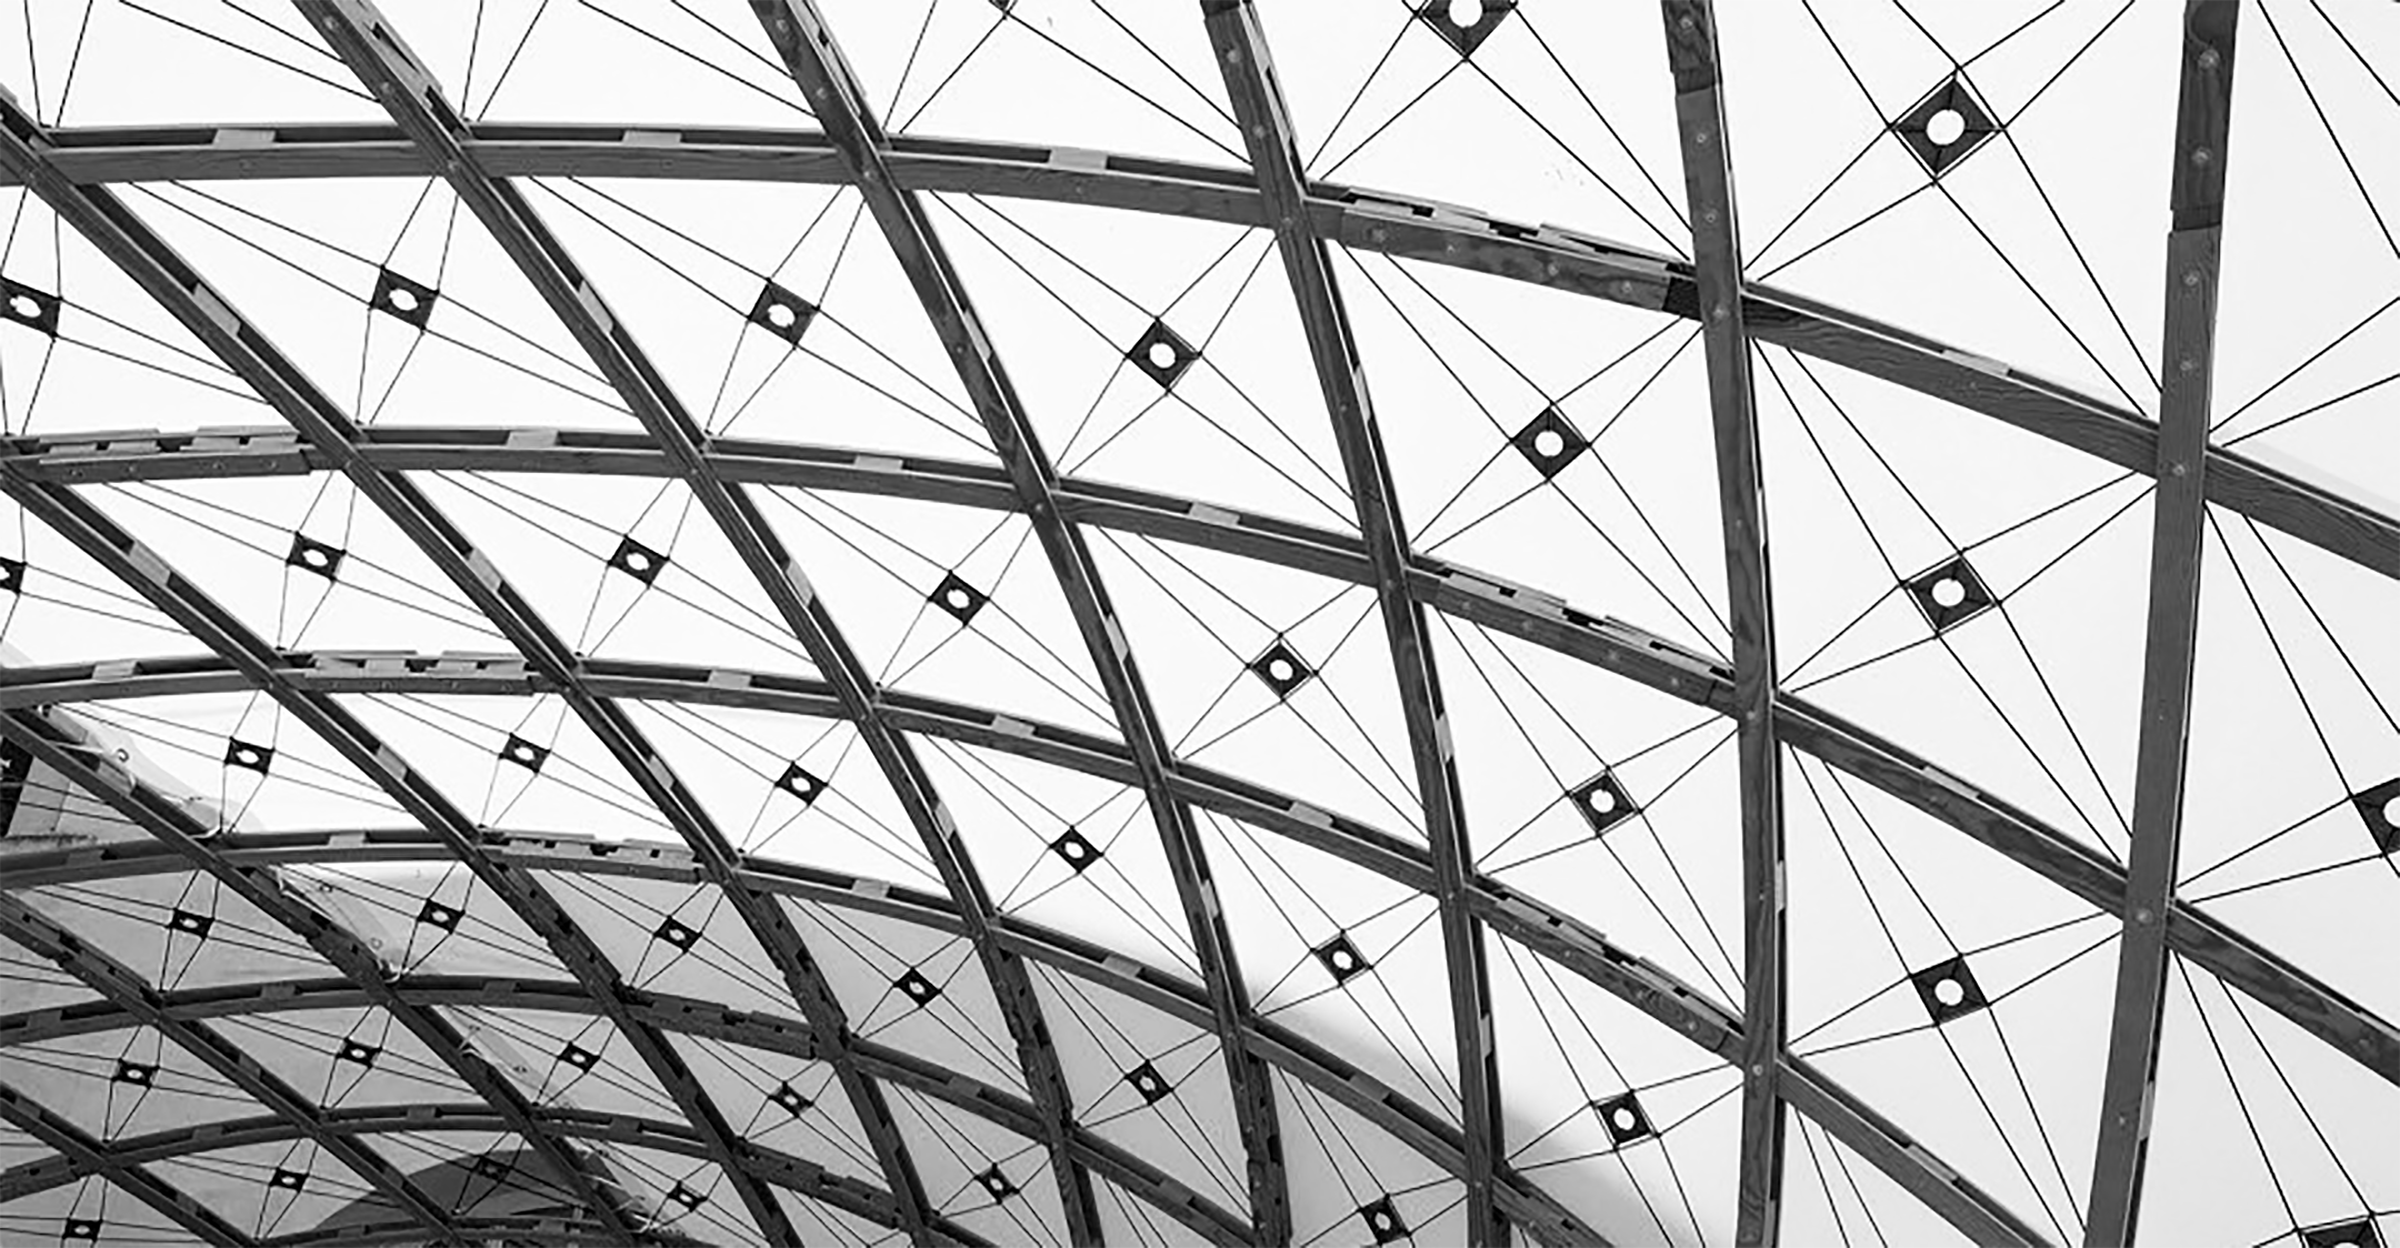
\includegraphics[width=30cm]{fav_nb.png}}};
		% image mask
		\path[fill,white,opacity=1] 
			(PPtl) -- (SPtr) -- (SPtr |- MBtr) --  (MBtr -| PPtr) -- (PPbr) -- (PPbl) -- (PPtl);
		% main bar
		\path[fill,black,opacity=1]  (MBbl) rectangle (MBtr -| PPtr);
		\node[anchor=east, xshift=-\MainTextXMargin, yshift=\MainBarHeight/2] at (MBbr){%
			\fbox{\parbox[b]{16cm}{\raggedleft\color{white}\tfelastica ELASTIC}}};
		\node[anchor=east, xshift=-\MainTextXMargin, yshift=-\MainBarHeight/2] at (MBbr){%
			\fbox{\parbox[b]{16cm}{\raggedleft\color{secondary}\tfgridshell GRIDSHELL}}};
	\end{tikzpicture}
	%
	\begin{tikzpicture}[remember picture, inner sep=0pt]
		% author bar
		\node[anchor=south east, xshift=-\MainTextXMargin, yshift=\AuthorYMargin] at (PGbr -| PPtr){%
			\fbox{\hbox{\tfauthor Lionel du Peloux}}};
		\coordinate (AHbl) at (current bounding box.south west);
		\coordinate (AHbr) at (current bounding box.south east);
		\coordinate (AHtl) at (current bounding box.north west);
		\coordinate (AHtr) at (current bounding box.north east);
		\path[fill,black] ([yshift=-2mm]AHbl) rectangle ([yshift=-4mm]AHbr);
		% year
		\node[anchor=center, yshift=\MainBarHeight/2] (MByear) at (MBbr -| PPt){%
			\fbox{\hbox{\color{white}\tfyear 2017}}};
		% phd
		\node[anchor=center, xshift=-\MainBarStepWidth/2, rotate=90] (MBphd) at (MByear -| SPtl){%
			\fbox{\hbox{\color{white}\tfphd PhD}}};
		\pgfresetboundingbox
		\path[use as bounding box] (0,0);
	\end{tikzpicture}
	%
	\begin{tikzpicture}[remember picture, overlay, inner sep=0pt]
		% abstract
		\node[anchor=south west, xshift=0.5cm, yshift=0.5cm] at (CAbl){%
			\fbox{\parbox[b]{16cm}{%
			\tftxt%
			\begin{multicols}{2}%
				An \emph{elastic gridshell} is a freeform structure, generally doubly curved, but formed out through the reversible deformation of a regular and initially flat structural grid. Building curved shapes that may seems to offer the best of both worlds~: shell structures are amongst the most performant mechanically speaking while planar and orthogonal constructions are much more efficient and economic to produce than curved ones. This ability to \textquote{form a form} efficiently is of peculiar importance in the current context where morphology is a predominant component of modern architecture, and envelopes appear to be the neuralgic point for building performances.

				The concept was invented by Frei Otto, a German architect and structural engineer who devoted many years of research to gridshells. In 1975 he designed the Multihalle of Mannheim, a \SI{7500}{m^2} wooden shell which demonstrated the feasibility of this technology and made it famous to a wide audience. However, despite their potential, very few projects of this kind were built after this major realization. And for good reason, the resources committed at that time cannot guarantee the replicability of this experiment for more standard projects, especially on the economic level. Moreover, the technics and methods developed by Otto's team in the 1960s have mostly fall into disuse or are based on disciplines that have considerably evolved. New materials, such as composite materials, have recently emerged. They go beyond the limitations of conventional materials such as timber and offer at all levels much better technical performances for this kind of application. Finally, it should be noted that the regulatory framework has also deeply changed, bringing a certain rigidity to the penetration of innovations in the building industry. Therefore, the design of gridshells arises in new terms for current architects and engineers and comes up against the inadequacy of existing tools and methods.

				In this thesis, which marks an important step in a personal research adventure initiated in 2010, we try to embrace the issue of the design of elastic gridshells in all its complexity, addressing both theoretical, technical and constructive aspects. In a first part, we deliver a thorough review of this topic and we present in detail one of our main achievements, the ephemeral cathedral of Créteil, built in 2013 and still in service. In a second part, we develop an original discrete beam element with a minimal number of degrees of freedom adapted to the modeling of bending and torsion inside gridshell members with anisotropic cross-section. Enriched with a ghost node, it allows to model more accurately physical phenomena that occur at connections or at supports. Its numerical implementation is presented and validated through several test cases. Although this element has been developed specifically for the study of elastic gridshells, it can advantageously be used in any type of problem where the need for an interactive computation with elastic rods taking into account flexion-torsion couplings is required.
			\end{multicols}%
			% 
			}}
		};
	\end{tikzpicture}
}
\hbox{}
% \begin{figure}
% 	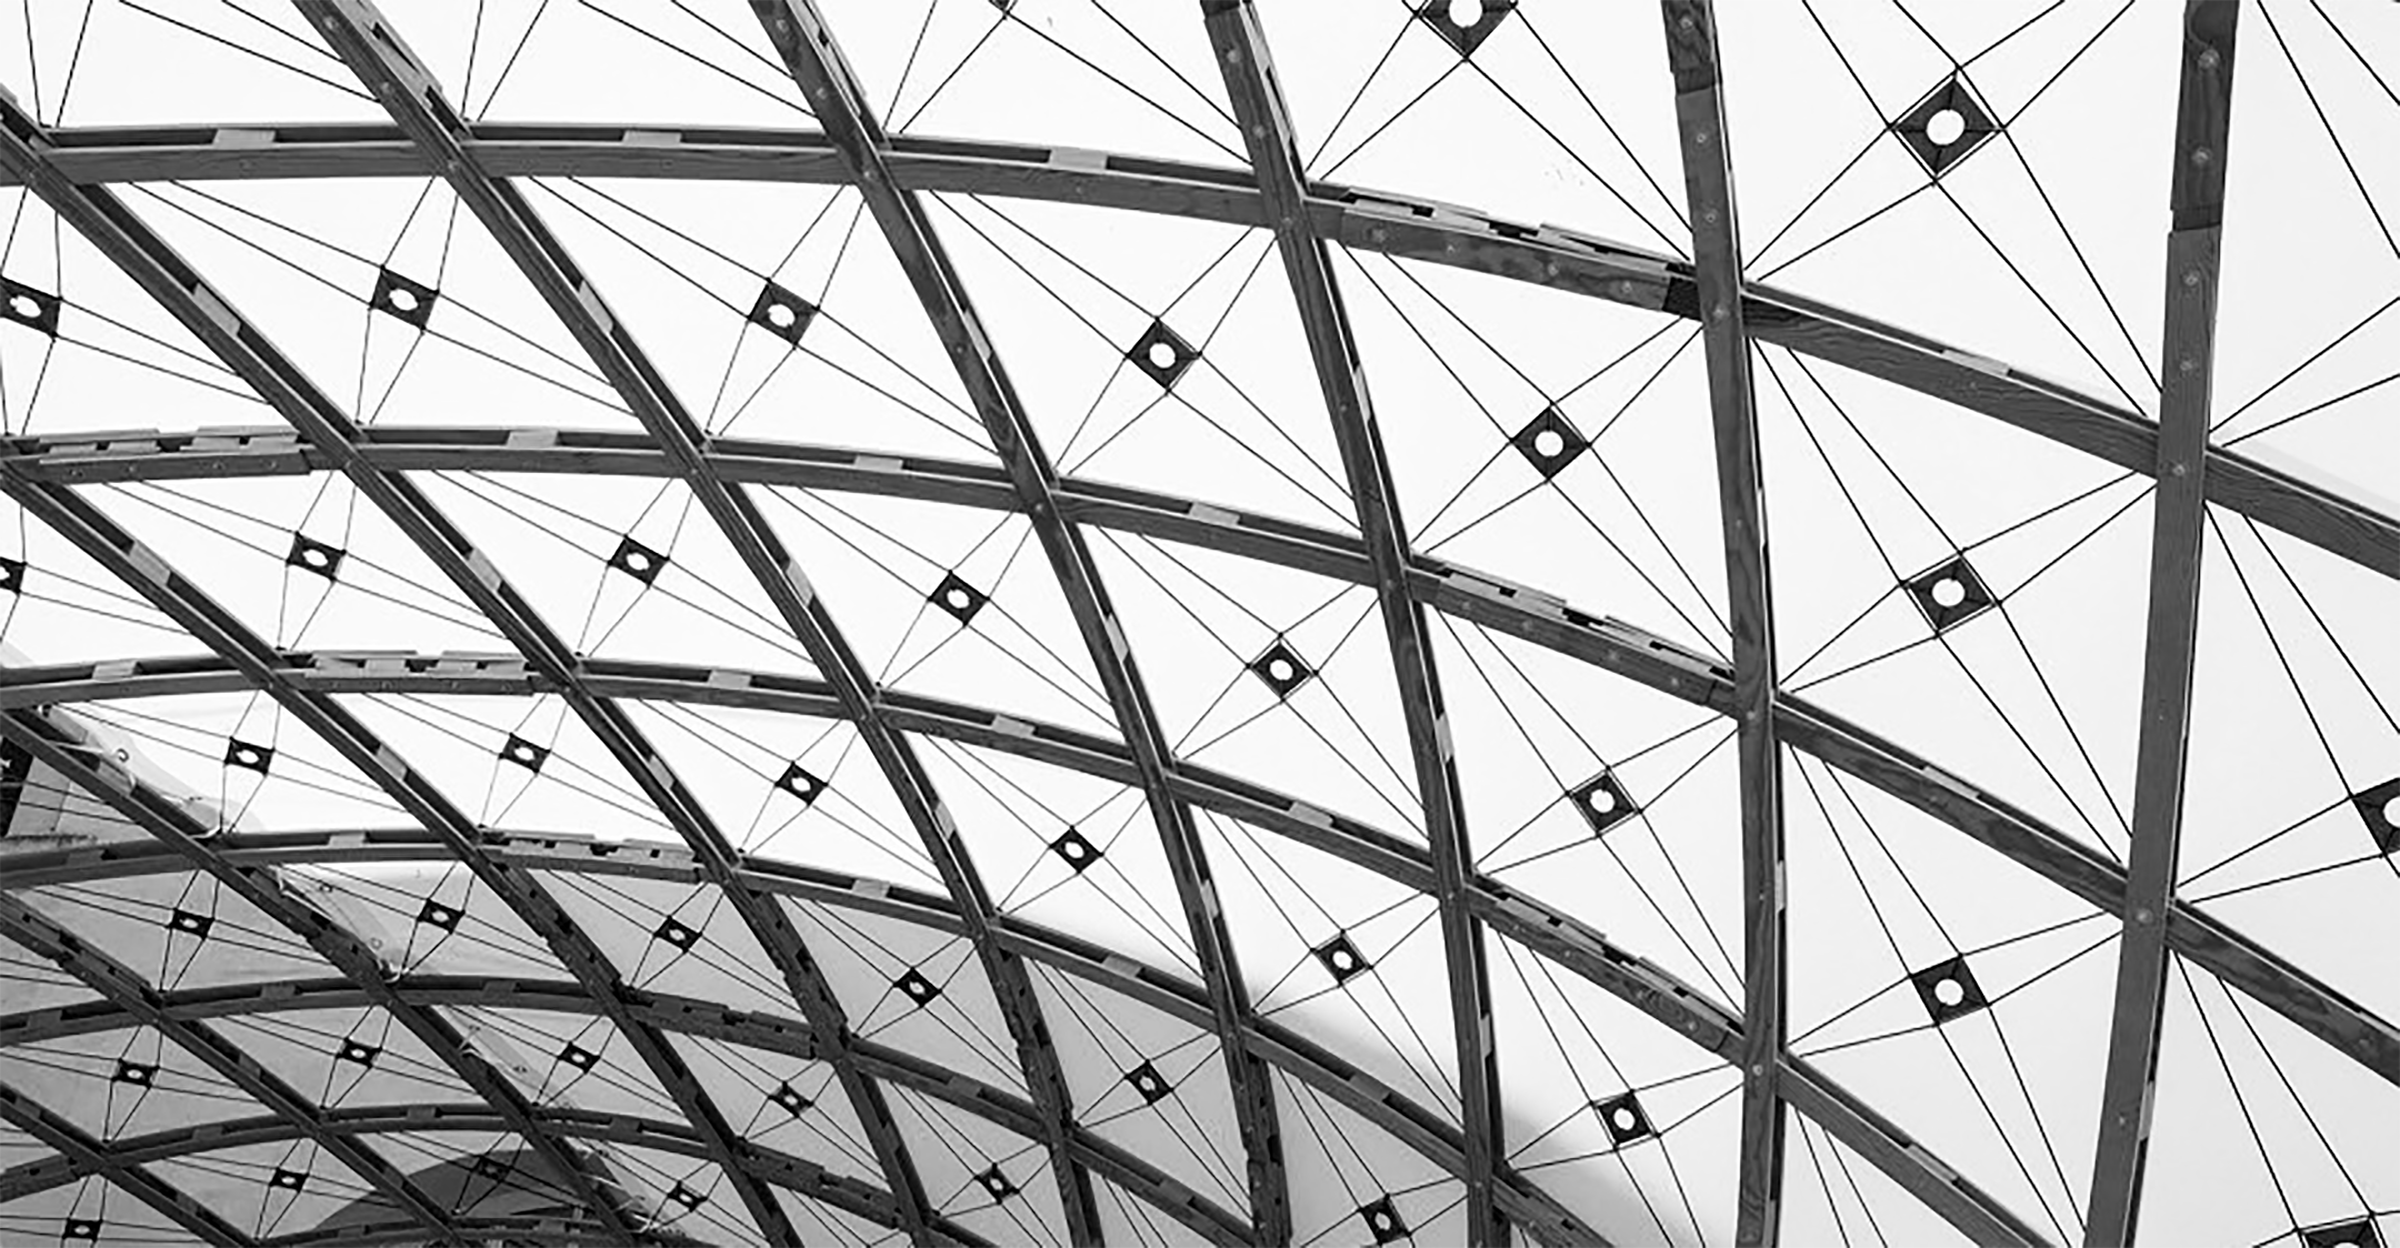
\includegraphics{fav_nb.png}
% \end{figure}

% \begin{titlepage}
% 	\begin{center}
% 	
\includegraphics[width=6cm]{head/logo_upe}\\
% 	\vspace{2cm}
% 	\setstretch{1.5}
% 	{\Large Thèse de doctorat} \\
% 	{\large École doctorale~: Science, Ingénierie et Environnement}\\
% 	{\large Spécialité~: Structures et Matériaux}\\
% 	\vspace{18pt}
% 	{\Large Présentée par}\\
% 	{\large \myauthor}
	
% 	\vfill
	
% 	\setstretch{2}
% 	{\ttfamily
% 	{\bfseries\huge  Modeling of bending-torsion couplings in active-bending structures}
% 	\\\vspace{12pt}
% 	{\Large Application to the design of elastic gridshells}
% 	}
	
% 	\vfill
% 	\setlength{\parskip}{0em}
% 	{\large Soutenue à l'Ecole Nationale des Ponts et Chaussées,\\\vspace{-10.0pt}le 20 décembre 2017, devant le jury composé de~:}
	
% 	\vspace{1.5cm}
	
% 	\setstretch{1.2}
% 	{\setlength{\tabcolsep}{0.5cm}\ra{1.0}
% 	\begin{tabular}{@{}>{}lll@{}}
% 	Président 		& Bernard MAURIN 			& Université Montpellier 2\\
% 	\addlinespace
% 	Rapporteurs 	& Sébastien NEUKIRCH 		& Université Pierre et Marie Curie\\
% 					 & Carlos LÁZARO 			& Universitat Politècnica de València\\
% 	\addlinespace
% 	Examinateurs	& Alberto PUGNALE 			& University of Melbourne\\
% 					 & Jean-François CARON 		& École des Ponts ParisTech\\
% 					 & Cyril DOUTHE 				& École des Ponts ParisTech\\
% 	\addlinespace
% 	Invité 			& Bernard VAUDEVILLE 		& T/E/S/S atelier d'ingénierie\\
% 	\addlinespace
% 	Directeur de thèse 	& Olivier BAVEREL 		& École des Ponts ParisTech\\
% 	\end{tabular}}
% 	\end{center}
% 	\end{titlepage}
	
	
\end{document}

